\documentclass{beamer}

\usepackage{hyperref,tikz,color,graphics}
\usepackage{bibentry}
\nobibliography*
% \usepackage{beamerthemesplit} // Activate for custom appearance

\title{Parasites: Can Little Things Eat Big Things?}
\author{Nick}
\date{\today}
\usecolortheme{rose}
\usetheme{CambridgeUS}

\begin{document}

\frame{\titlepage}

\frame{\tableofcontents}

\section{Motivation}

\begin{frame}
\frametitle{Parasitism in Food Webs}
\begin{itemize}[<+->]
\item  Underrepresentation
\item  Novel, complex, and specific
\item  Place in Food Webs
\end{itemize}
\end{frame}

\begin{frame}
\frametitle{Past Work}
\begin{itemize}[<+->]
\item  Effect of Adding Parasites \footnote{\tiny\bibentry{Dunne2013}}
\item  Importance of Body Size Ratios \footnote{\tiny\bibentry{Brose2006}}
\item  An Inverse Niche Model \footnote{\tiny\bibentry{Warren2010}}
\end{itemize}
\end{frame}

\begin{frame}
\frametitle{Research Goals}
\begin{itemize}[<+->]
\item Niche Model vs. Inverse Niche Model(s)
\item  Dynamical Simulations
\item  Concommitant (Incidental) Predation
\end{itemize}
\only<3>{
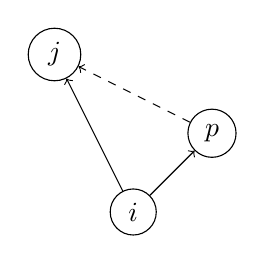
\begin{tikzpicture}
\node[draw,circle] at (0,0) (j) {$j$};
\node[draw,circle] at (1,-2) (i) {$i$};
\node[draw,circle] at (2,-1) (p) {$p$};
\draw[->] (i)--(j);
\draw[->] (i)--(p);
\draw[->,dashed] (p)--(j);
\end{tikzpicture}
}
\end{frame}


\section{Food Web Models}

\begin{frame}
\frametitle{Empirical Data}
\begin{itemize}
\item Bahia San Quintin, Estero de Punta Banda (bahia,punta)
\only<1>{
\begin{itemize}
\item \href{http://proesteros.cicese.mx/humedalesbc.html}{Pics}
\item \href{http://www.youtube.com/watch?v=9lknc3VuJhA&t=5m21s}{View}
\item \href{https://www.youtube.com/watch?v=9lknc3VuJhA&t=15m33s}{Bird}
\end{itemize}
}
\item Carpinteria Salt Marsh (carp)
\only<2>{
\begin{itemize}
\item \href{http://carpinteria.ucnrs.org/images/gallery/watershed1.JPG}{Aerial}
\item \href{http://carpinteria.ucnrs.org/images/gallery/MARSH6.JPG}{Close}
\item \href{http://carpinteria.ucnrs.org/images/gallery/lasthenia.jpg}{Flowers}
\end{itemize}
}
\item Otago Harbor (otago)
\only<3>{
\begin{itemize}
\item \href{http://esapubs.org/archive/ecol/E092/173/metadata.htm\#rsrchdescs}{Map1}
\item \href{https://www.google.com/maps/@-45.83,170.66,10000m/data=!3m1!1e3?hl=en}{Map2}
\item \href{http://expatedna.com/wp-content/uploads/2012/06/sara-guest-post-2.jpg}{Far}
\end{itemize}
}
\item Sylt Tidal Basin (sylt)
\only<4>{
\begin{itemize}
\item \href{http://esapubs.org/Archive/ecol/E092/172/metadata.htm\#rsrchdescs}{Map1}
\item \href{https://www.google.com/maps/@54.99,8.55,25000m/data=!3m1!1e3?hl=en}{Map2}
\item \href{https://www.google.com/maps/@55.0814776,8.5206852,3a,75y,199.65h,71.06t/data=!3m6!1e1!3m4!1s_cH9rZdhYN2rK1JJO2Nw0A!2e0!7i13312!8i6656?hl=en}{Road}
\end{itemize}
}
\item Flensburg Fjord (flens)
\only<5>{
\begin{itemize}
\item \href{http://esapubs.org/Archive/ecol/E092/174/metadata.htm\#rsrchdescs}{Map1}
\item \href{https://www.google.com/maps/@54.795706,9.7782185,1476m/data=!3m1!1e3?hl=en}{Map2}
\item \href{https://www.google.com/maps/@55.0814776,8.5206852,3a,75y,199.65h,71.06t/data=!3m6!1e1!3m4!1s_cH9rZdhYN2rK1JJO2Nw0A!2e0!7i13312!8i6656?hl=en}{Road}
\end{itemize}
}
\end{itemize}
\end{frame}

\begin{frame}
\frametitle{Empirical Data}
\begin{tabular}{|r| c c c c c |}
\hline
Parasitic Webs&$S$&$C$&$S_{free}$&$S_{free}$&$S_{basal}$\\
\hline
bahia&141&.092 &.35&.65&.06\\
carp&154&.085&.36&.64&.06\\
punta&185&.084&.37&.63&.05\\
flens&109&.073&.38&.62&.06\\
otago&117&.077&.15&.85&.03\\
sylt&147&.079&.20&.80&.04\\
\hline
\hline
Free Webs&$S$&$C$&$S_{par}$&$S_{free}$&$S_{basal}$\\
\hline
bahia&80&.085 &0&1&.11\\
carp&91&.096&0&1&.10\\
punta&106&.099&0&1&.08\\
flens&56&.11&0&1&.11\\
otago&94&.085&0&1&.04\\
sylt&117&.073&0&1&.05\\
\hline
\end{tabular}
\end{frame}

\begin{frame}
\frametitle{Empirical Data}
\begin{columns}[c]
\column{0.2\textwidth}
\tiny
\begin{tabular}{r|c c c c c c c c c c c}
\input{variableKey.textab}
\end{tabular}
\column{0.8\textwidth}
\only<1>{\includegraphics[width =\textwidth]{corMapPear.jpg}}
\only<2>{\includegraphics[width=\textwidth]{corMapSpear.jpg}}
\end{columns}
\end{frame}


\begin{frame}
\frametitle{Inverse Niche Models}
\only<1>{
\begin{tikzpicture}
\draw (0,0)--(10,0)
node[anchor = west] {$n$};
\draw (0,.2)--(0,-.2)
node[anchor = north] {$0$};
\draw (10,.2)--(10,-.2)
node[anchor = north] {$1$};
%Predator
\fill (7,0) circle (.07) 
node[anchor = north]  {$n_j$};
%Predator Diet
\draw (7,0)--(7,.75)--(2,.75)--(2,.5);
\draw (.3,0) -- (.3,.5) -- (3.7,.5) -- (3.7,0);
\draw[dashed] (2,.5) -- (2,0) 
node[anchor = south east] {$c_j$};
\draw[<->] (.3,-.5) -- (3.7,-.5)
node[fill=white,pos = 0.5] {$r_j$}; 
\draw[dashed] (.3,0)--(.3,-.55);
\draw[dashed] (3.7,0)--(3.7,-.55);
%Prey
\fill (3,0) circle (.07) 
node[anchor = north west]  {$n_i$};
\draw(4.2,-2) circle (.3)
node {$i$};
\draw[->] (4.5,-2) -- (5.5,-2);
\draw(5.8,-2) circle (.3)
node {$j$};
\end{tikzpicture}
}
\only<2->{
\begin{tikzpicture}
\draw (0,0)--(10,0)
node[anchor = west] {$n$};
\draw (0,.2)--(0,-.2)
node[anchor = north] {$0$};
\draw (10,.2)--(10,-.2)
node[anchor = north] {$1$};
%Host
\fill (6,0) circle (.07) 
node[anchor = north]  {$n_i$};
%Predator Diet
\draw (7,0.5)--(7,.75)--(2,.75)--(2,0);
\draw (5.3,0) -- (5.3,.5) -- (8.7,.5) -- (8.7,0);
\draw[dashed] (7,.5) -- (7,0) 
node[anchor = south east] {$c_p$};
\draw[<->] (5.3,-.5) -- (8.7,-.5)
node[fill=white,pos = 0.5] {$r_p$}; 
\draw[dashed] (5.3,0)--(5.3,-.55);
\draw[dashed] (8.7,0)--(8.7,-.55);
%Parasite
\fill (2,0) circle (.07) 
node[anchor = north west]  {$n_p$};
\draw(4.2,-2) circle (.3)
node {$i$};
\draw[->] (4.5,-2) -- (5.5,-2);
\draw(5.8,-2) circle (.3)
node {$p$};
\end{tikzpicture}
}
\begin{itemize}
\item<3-> $n_p \sim U(\textcolor{red}{a,b})$
\item<4-> $y_p \sim \text{Beta}(1,\textcolor{red}{\beta_p})$
\item<5-> $r_p \sim \textcolor{red}{(1-n_p)} \cdot y_p$
\item<6-> $c_{p}\sim U(\max{(n_p,r_p/2)},1-r_p/2)$
\end{itemize}
\end{frame}

\begin{frame}
\frametitle{Inverse Niche Models: Further Issues}
\begin{itemize}
\item <1-> Types of links; sub-web connectances
\item <2-> Diet intersections with parasitic niches
\item <3-> Scale dependent errors vs. Parasitic errors
\item <4-> Low(?) parasitic resolution
\end{itemize}
\end{frame}

\begin{frame}
\frametitle{Proposed Models}
All at once models:
\begin{tabular}{|r |l|}
\hline
&Description\\
\hline
Model 0& Plain Niche Model\\
Model 1& Random parasites; correct bias; eat below\\
Model 2& Random parasites; correct bias; eat above\\
\hline
\end{tabular}

Adding to niche web models:
\begin{tabular}{|r|c c c c|}
\hline
&min($n_p$)&max($n_p$)&Invert Parasites&Match $C_{fp}$\\
\hline
Model 3 & 0 & 1 & no & no\\
Model 4 & 0 & 1 & no & yes\\
Model 5 & 0 & 1 & yes & no\\
Model 6 & 0 & 1 & yes & yes\\
Model 7 & 0.7 & 0.9 & no & yes\\
Model 8 & 0.1 & 0.3 & yes & yes\\
\textcolor{red}{Model 9} & 0.1 & 0.3 & yes & no\\
\textcolor{red}{Model 10} & 0.7 & 0.9 & no & no\\
\hline
\end{tabular} 
\end{frame}

\begin{frame}
\frametitle{(Selected) Results of models}
\only<1>{
\includegraphics[width=.9\textwidth]{propPlot1.jpg}
}
\only<2>{
\includegraphics[width=.9\textwidth]{propPlot2.jpg}
}
\only<3>{
\includegraphics[width=.9\textwidth]{propPlot3.jpg}
}
\only<4>{
\includegraphics[width=.9\textwidth]{propPlot4.jpg}
}
\only<5>{
\includegraphics[width=.9\textwidth]{propPlot5.jpg}
}
\only<6>{
\includegraphics[width=.9\textwidth]{propPlot6.jpg}
}
\end{frame}

\begin{frame}
\frametitle{Empirical Data Revisited}
Generalities of Free-Living Consumers and Parasites
\begin{tabular}{|r| c c |c|}
\hline
Web& $G_{f},(n_f)$ & $G_p,(n_p)$ &  P-value\\
\hline
bahia&0.8984,(83)&1.355,(49)&\textcolor{red}{.0091}\\
carp&1.012,(88)&1.161,(56)&.3835\\
punta&1.173,(108)&0.8570,(68)&\textcolor{red}{.0310}\\
flens&1.190,(62)&0.8595,(41)&.0714\\
otago&1.040,(96)&1.012,(17)&.8857\\
sylt&.9019,(112)&1.586,(29)&\textcolor{red}{.0036}\\
\hline
\end{tabular}
\end{frame}

\begin{frame}
\frametitle{Empirical Data Revisited}
\begin{itemize}[<+->]
\item Independence
\item Empirical
\item Matching Dunne et al 2013.
\end{itemize}
\end{frame}

\section{Identifying Parasites}

\begin{frame}
\frametitle{Empirical Data Revisited; Local}
$P$-values for testing $\mu_{free} - \mu_{para}\neq0$ for each property:\vspace{.25in}

\tiny{
\begin{tabular}{|r| c c c c c c|}
\hline
\input{pValsAllProps2.textab}
\hline
\end{tabular}}
\end{frame}

\begin{frame}
\frametitle{A Classification Tree}
\begin{itemize}[<+->]
\item Binary Splits
\item 4 classes
\item Species Overlap?
\item How to use?
\end{itemize}
\end{frame}

\begin{frame}
\frametitle{A Classification Tree}
\begin{tikzpicture}
\tikzstyle{every node}=[draw,rectangle]
\node [] at (0,0) (A) {\tiny
\begin{tabular}{c|c}
Class&Count\\
\hline
1&310\\
2&79\\
3&160\\
4&260\\
\hline
error&61.7\%\\
\end{tabular}
};
\node at (-1.5,-3) (B) {\tiny\begin{tabular}{c|c}
Class&Count\\
\hline
1&213\\
2&3\\
3&22\\
4&2\\
\hline
error&11.2\%\\
\end{tabular}
};
\node at (6,0) (C) {\tiny\begin{tabular}{c|c}
Class&Count\\
\hline
1&97\\
2&76\\
3&138\\
4&258\\
\hline
error&54.6\%\\
\end{tabular}
};
\node at (1.5,-3) (D) {\tiny\begin{tabular}{c|c}
Class&Count\\
\hline
1&18\\
2&3\\
3&2\\
4&119\\
\hline
error&16.1\%\\
\end{tabular}
};
\node at (6,-3) (E) {\tiny\begin{tabular}{c|c}
Class&Count\\
\hline
1&79\\
2&73\\
3&136\\
4&139\\
\hline
error&67.4\%\\
\end{tabular}
};
\node at (2,-6) (F) {\tiny\begin{tabular}{c|c}
Class&Count\\
\hline
1&59\\
2&64\\
3&119\\
4&27\\
\hline
error&55.8\%\\
\end{tabular}
};
\node at (7.5,-6) (G) {\tiny\begin{tabular}{c|c}
Class&Count\\
\hline
1&20\\
2&9\\
3&17\\
4&112\\
\hline
error&29.1\%\\
\end{tabular}
};
\draw[->] (A)-- node [pos = 0.5,fill =white] {\tiny$swTL <2.91$} (B);
\draw[->] (A)--node [pos = 0.5,fill =white] {\tiny$swTL \geq2.91$}(C);
\draw[->] (C)--node [pos = 0.5,fill =white] {\tiny$\langle genPred \rangle <.124$}(D);
\draw[->] (C)--node [pos = 0.5,fill =white] {\tiny$\langle genPred \rangle \geq.124$}(E);
\draw[->] (E)--node [pos = 0.5,fill =white] {\tiny$\langle genPred \rangle <2.38$}(F);
\draw[->] (E)--node [pos = 0.5,fill =white] {\tiny$\langle genPred \rangle \geq 2.38$}(G);
\only<1>{\node [blue] at (-1,-5) (Key) {\tiny
\begin{tabular}{c |l}
Number&Class\\
\hline
1&Ecto. Inv.\\
2&Ecto. Vert.\\
3&Endotherm\\
4&Parasite
\end{tabular}};}
\only<2>{
\node [blue] at (-1.2,-5) {\tiny
\begin{tabular}{c| l| l}
Split& Error & Var. Exp.\\
\hline
0&.617&-\\
1&.418&.323\\
2&.418&0\\
3&.304&.184\\
\end{tabular}
};}
\end{tikzpicture}
\end{frame}

\begin{frame}
\frametitle{Classification Tree + Niche Model}
\begin{itemize}[<+->]
\item Generate Niche Model
\item Parasites from Classification Tree or Randomly
\item To do:
\begin{itemize}[<+->]
\item Properties of chosen classes
\item Training data?
\item Classification on ONM/INM
\item Consumer-Resource body size ratios
\end{itemize}
\end{itemize}
\end{frame}

\section{Numerical Experiments}

\begin{frame}
\frametitle{Numerical Experiments}
\begin{itemize}[<+->]
\item Constant body mass ratios already studied
\item What is maximum fraction of parasites allowed?
\item Where do empirical webs fit in the pattern?
\item How do concomittant links affect that pattern?
\end{itemize}
\end{frame}

\begin{frame}
\frametitle{Dynamical Model}
\begin{equation}\label{eq:ATNAAAI}
\begin{array}{r l}
\frac{dB_{i}}{dt} &= r_{i}\left(1-\frac{\sum_{j\in \text{basal}}B_{j}}{K}\right)B_{i}\\[1ex]
& - x_{i}B_{i}\\[1ex]
& + \phi_ix_{i}B_{i}\sum_{j \in \text{diet}(i)}F_{ji}y\\[1ex]
&- \phi_i\sum_{j \in \text{pred}(i)}x_{j}B_{j}F_{ij}y/e_{ij} \\[1ex]
&-(1-\phi_i)\{\text{Concomittant Losses}\}
\end{array}
\end{equation}

and

\begin{equation}\label{eq:FRAAAI}
F_{ij} = \frac{\omega_{ij}B_{i}^{h}}{B_{0}^{h}+ \sum_{k\in \text{diet}(j)}\omega_{kj}B_{k}^{h}}
\end{equation}
\end{frame}

\begin{frame}
\frametitle{Body Mass Ratios\footnote{\tiny\bibentry{Brose2006}}}
\only<1>{
\begin{columns}[c]
\column{0.55\textwidth}
\includegraphics[width=\textwidth]{BMR.jpg}
\column{0.45\textwidth}
\begin{tabular}{r|c}
Type&Median\\
\hline
Ecto. Inv.&72.1 (318)\\
Ecto. Vert.&887\\
Endo.&2160\\
Para.&$1.77\times10^{-6}$
\end{tabular}
\end{columns}
}
\only<2>{
\begin{columns}[c]
\column{0.4\textwidth}
\includegraphics[width=\textwidth]{BMR_BWM.jpg}
\column{0.6\textwidth}
\begin{tabular}{r|c}
Type&Median\\
\hline
Ecto. Inv.&14\\
Ecto. Vert.&398\\
\end{tabular}
\end{columns}
}
\only<3->{
\begin{itemize}[<+->]
\item Parasites are small.
\item To parameterize: $M = Z^{TL}$.
\end{itemize}
}
\end{frame}

\begin{frame}
\frametitle{Body Size Ratios \& Body Sizes}
\only<1>{
\includegraphics[width=.8\textwidth]{bstl.jpg}
}
\only<2>{
\includegraphics[width=.8\textwidth]{bsrtl.jpg}
}
\end{frame}


\begin{frame}
\frametitle{Dynamical Model: Next Steps}
\begin{itemize}[<+->]
\item Allometric scaling for parasites
\item Concomittant Losses
\end{itemize}
\end{frame}

\bibliographystyle{siam}
\nobibliography{/Users/Nick/Documents/Papers/Bibs/Bib_green.bib}
\end{document}
